% 2011 年四川卷文科第 7 题：正六边形 ABCDEF，求 \vec{BA}+\vec{CD}+\vec{EF}。
% 来源 PDF：普通高考/2011/2011四川文.pdf，SHA-256 9df4a6b69bb06bfab2f7d7ee0e7fcc50ae547f226260996d7a060c31ad14e64a。
% 原页：第 1 页（A3 三栏）第 1 栏下部，书页码 703。
% 重绘依据：照原页——上边 DE 水平、下边 BA 水平，D 在左上、E 在右上、C 在左、F 在右，
%   B 在左下、A 在右下；按正六边形作图，原页不画顶点圆点、不画对角线。
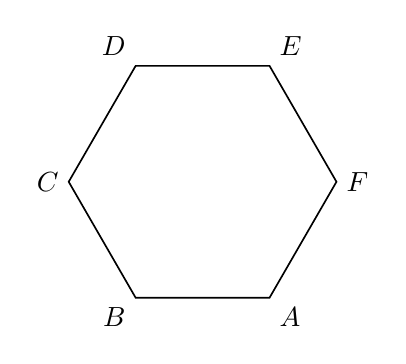
\begin{tikzpicture}[scale=1.7, >=stealth, semithick]
  \coordinate (A) at (0.5,-0.8660);
  \coordinate (B) at (-0.5,-0.8660);
  \coordinate (C) at (-1,0);
  \coordinate (D) at (-0.5,0.8660);
  \coordinate (E) at (0.5,0.8660);
  \coordinate (F) at (1,0);
  \draw (A) -- (B) -- (C) -- (D) -- (E) -- (F) -- cycle;
  \node at (A) [below right] {$A$};
  \node at (B) [below left] {$B$};
  \node at (C) [left] {$C$};
  \node at (D) [above left] {$D$};
  \node at (E) [above right] {$E$};
  \node at (F) [right] {$F$};
\end{tikzpicture}
